


\section{Scenegraphs and Physics}

Animation is usually based upon VJoints, arranged into tree shaped scenegraphs.
This provided the interface between, on the one hand, rendering systems like those
from the hmi/graphics packages and, on the other hand, animation systems based upon interpolators, procedural animation,
or physics based simulation.

 Our animation structure is such that it supports splitting the rendering and animating processes into two separate threads. To allow this (and in the future possibly to allow multiple remote visualizations of the animation process running on a server), we separate the rendering and animation VJoint scene graphs (see Figure \ref{figuresg}). The local transform of the nodes under animation root is coupled to the render scene at its initialization. This coupling is many-to-one: one or more animation VJoints can steer a single render node. For example: a render node containing a deformable mesh for a humanoid is steered by a tree of animation VJoints representing the skeleton that steers the mesh. The animation tree is coupled to the render tree using the VJoint rotation/translation buffers: setting the rotation or translation of a animation tree VJoint directly sets the rotation in the corresponding render node. If animation and rendering occurs in different threads, access to the animation tree should be synchronized. This prevents the render thread reading partial information from the animation scene while it is still being updated by the animation thread. Typically the animation processes use copies of parts of the animation tree locally in time consuming animation processes and then uses a synchronized copy action to copy the resulting VJoint transformations to the animation scene. The render thread uses a synchronized action to calculate the global render node transformations from rotations in the animation tree (see also Figure \ref{threads}).

For a typical linking scenario see this \href{\hmianimationreportdir/typical_scenegraph.pdf}{scenegraph linking example}

\subsection{Example: animation algorithm in Elckerlyc}
The AnimationPlayerManager manages the animation proces in Elckerlyc. It contains an AnimationPlayer for each animated virtual human. It uses 3 copies of the joint tree of this humanoid: cur, prev, next, representing the joint rotations at $t$, $t-1$ and $t+h$ respectively. vjAni represents the root VJoint of the human in the animation joint tree. Animation is executed as follows:
\begin{enumerate}
\item run all animation players, in each animation player:
\begin{enumerate}
\item copy cur to prev, next to cur
\item run all procedural animations on next 
\item using prev, next and cur, calculate and apply the forces and torques generated by the kinematic motion to the human's physical body
\end{enumerate}
\item do a physics step
\item copy the physical body rotations to cur
\item copy the rotations of curr and its children to vjAni (and its children)
\end{enumerate}

\subsection{Synchronisation}
Acces to the VJoints in the Animation root should be synchronized to the animation sync:
\begin{verbatim}
synchronized(AnimationSync.getSync())
{
	do something with VJoints in animation root
}
\end{verbatim}
Access to objects controlled by physical simulation should be synchronized to the physics sync:
\begin{verbatim}
synchronized(PhysicsSync.getSync())
{
	access physical objects
}
\end{verbatim}

\begin{figure}
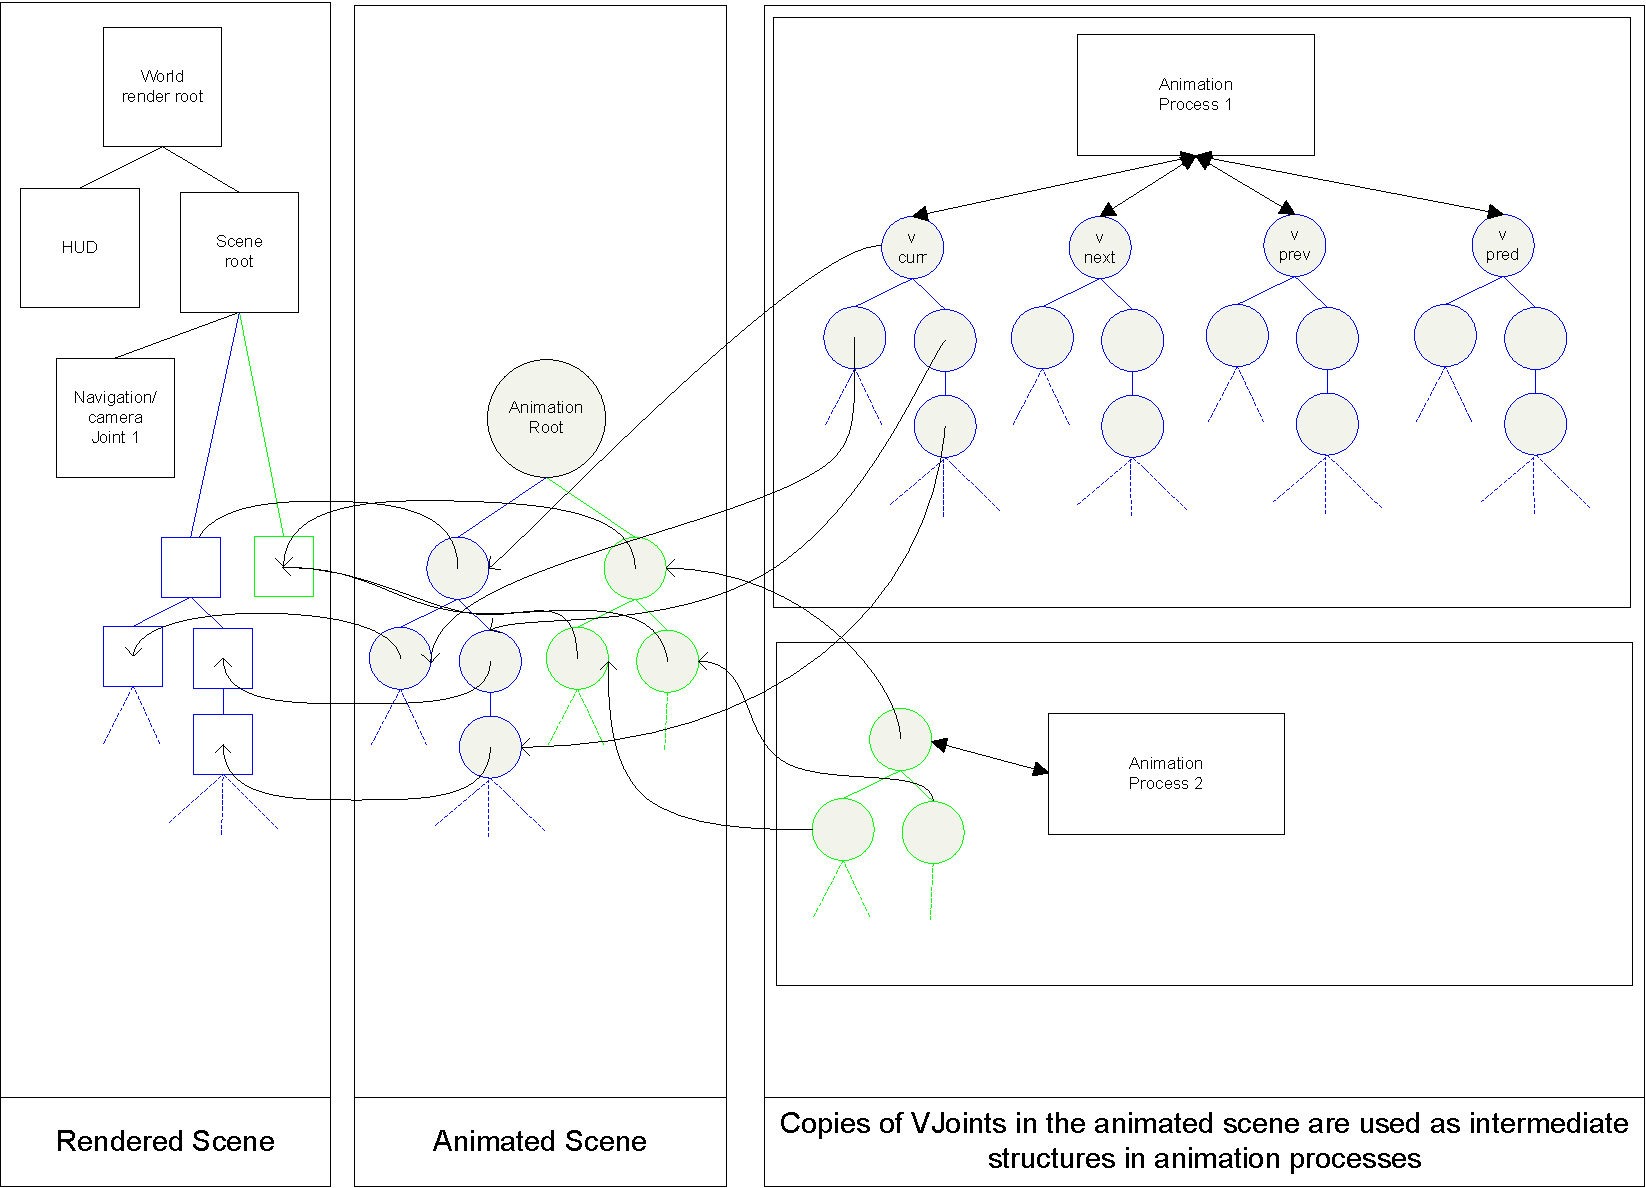
\includegraphics[width=13cm]{\hmianimationreportdir/typical_scenegraph}
\caption{\label{figuresg}Typical scenegraph layout}
\end{figure}

\begin{figure}
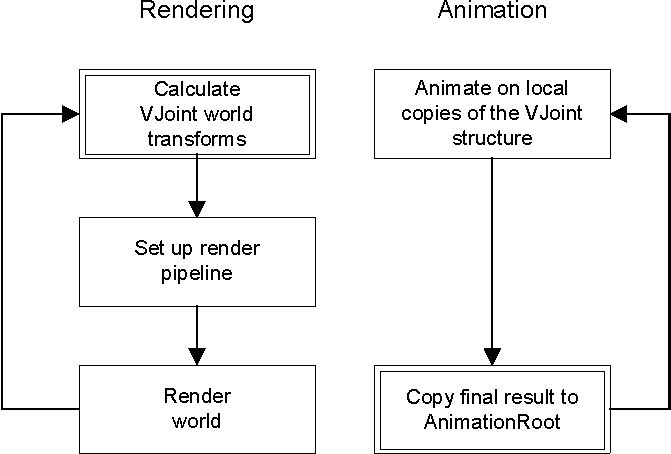
\includegraphics{\hmianimationreportdir/threads-crop}
\caption{\label{threads}Animation and rendering loops running in different threads. The processes with double lines are synchronized to each other.}
\end{figure}


